%================================================
% PACKAGES AND THEMES
%================================================
\documentclass[t,aspectratio=169,xcolor=dvipsnames]{beamer}

\usetheme{SimplePlusAIC}

\usepackage{graphicx}
\usepackage{booktabs}
\usepackage{svg}
\usepackage{tcolorbox}
\usepackage{tikz}
\usetikzlibrary{shapes.geometric, arrows, positioning, fit, calc}
\usepackage{makecell}
\usepackage{listings}

\newcommand*{\defeq}{\stackrel{\text{def}}{=}}
\usepackage{setspace}
\usepackage[T1]{fontenc}
\usepackage{helvet}
\usepackage{amsmath}
\usepackage{ragged2e}
\usepackage{gensymb}

\usepackage[svgnames,table]{xcolor}
\arrayrulecolor{black}
\setlength{\arrayrulewidth}{0.20mm}
\renewcommand{\arraystretch}{1.35}

\newcommand{\tem}[1]{\textbf{\textcolor{red}{#1}}}

% Listings configuration
\lstset{
    basicstyle=\ttfamily\small,
    breaklines=true,
    columns=fullflexible,
    frame=none
}

%================================================
% TITLE PAGE
%================================================
\title[TLB \& Demand Paging]{TLB \& Demand Paging}
\subtitle{Week 9: Hit, Miss, dan Page Fault}
\author[lectura.id/course/os]{lectura.id/course/os}
\institute[ITERA]{Program Studi Teknik Informatika \\ Institut Teknologi Sumatera}
\date{\textcolor{nyublue}{2026}}

%================================================
% BEGIN DOCUMENT
%================================================
\begin{document}

\begin{frame}
    \titlepage
\end{frame}

\begin{frame}
    \frametitle{OUTLINE}
    \framesubtitle{Peta materi pertemuan ini}
    \small
    \begin{spacing}{1.15}
        \tableofcontents
    \end{spacing}
\end{frame}

\begin{frame}
    \frametitle{Capaian Pembelajaran}
    \framesubtitle{Tujuan setelah pertemuan selesai}
    \small
    \begin{enumerate}
        \item Menjelaskan mengapa page table biasa menyebabkan overhead akses memori.
        \item Memahami cara kerja TLB dan membedakan TLB hit vs TLB miss.
        \item Menghitung \textit{Effective Access Time} (EAT) berdasarkan hit rate TLB.
        \item Memahami konsep demand paging dan alur penanganan page fault.
        \item Membandingkan algoritma page replacement: FIFO, Optimal, dan LRU.
    \end{enumerate}
    \begin{exampleblock}{Fokus Kelas Ini}
        Kita fokus pada \tem{cara kerja TLB}, \tem{perhitungan EAT}, dan \tem{algoritma page replacement} secara step-by-step.
    \end{exampleblock}
\end{frame}

\begin{frame}
    \frametitle{Analogi: Perpustakaan \& Catatan Saku}
    \framesubtitle{Bayangkan kamu sedang mencari buku di perpustakaan...}
    \small

    \begin{columns}[T]
        \column{0.50\textwidth}
        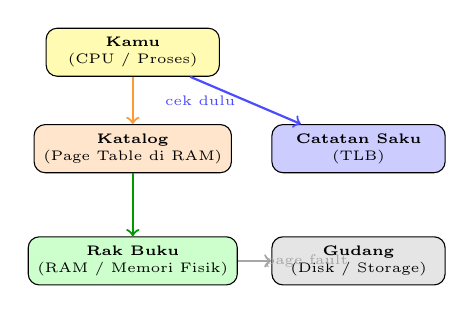
\begin{tikzpicture}[font=\tiny, node distance=0.4cm]
            % Katalog
            \node[draw, fill=orange!20, rounded corners, minimum width=2.2cm, minimum height=0.6cm, align=center] (catalog) {\textbf{Katalog} \\ (Page Table di RAM)};
            % Catatan saku
            \node[draw, fill=blue!20, rounded corners, minimum width=2.2cm, minimum height=0.6cm, align=center, right=0.5cm of catalog] (notes) {\textbf{Catatan Saku} \\ (TLB)};
            % Rak buku
            \node[draw, fill=green!20, rounded corners, minimum width=2.2cm, minimum height=0.6cm, align=center, below=0.8cm of catalog] (shelf) {\textbf{Rak Buku} \\ (RAM / Memori Fisik)};
            % Gudang
            \node[draw, fill=gray!20, rounded corners, minimum width=2.2cm, minimum height=0.6cm, align=center, below=0.8cm of notes] (warehouse) {\textbf{Gudang} \\ (Disk / Storage)};
            % Kamu
            \node[draw, fill=yellow!30, rounded corners, minimum width=2.2cm, minimum height=0.6cm, align=center, above=0.6cm of catalog] (you) {\textbf{Kamu} \\ (CPU / Proses)};

            \draw[->, thick, blue!70] (you) -- node[left, font=\tiny]{cek dulu} (notes);
            \draw[->, thick, orange!80] (you) -- (catalog);
            \draw[->, thick, green!60!black] (catalog) -- (shelf);
            \draw[->, thick, gray!70] (shelf) -- node[right, font=\tiny]{page fault} (warehouse);
        \end{tikzpicture}

        \column{0.46\textwidth}
        \vspace{0.2cm}
        \begin{itemize}
            \item \textbf{Katalog} = Page table: tahu lokasi semua buku, tapi harus didatangi dulu (lambat).
            \vspace{0.15cm}
            \item \textbf{Catatan saku (TLB)} = Kamu tulis lokasi buku yang \tem{sering dicari} — cek sini dulu sebelum ke katalog!
            \vspace{0.15cm}
            \item \textbf{Rak buku (RAM)} = Buku yang sudah ada di depanmu, langsung bisa dibaca.
            \vspace{0.15cm}
            \item \textbf{Gudang (Disk)} = Buku belum di rak $\rightarrow$ harus diambil dulu, \tem{butuh waktu lama}.
        \end{itemize}
    \end{columns}
\end{frame}

%================================================
% BAGIAN 1: REVIEW & MOTIVASI
%================================================
\section{Review \& Motivasi}

\begin{frame}
    \frametitle{Review: Paging \& Page Table}
    \framesubtitle{Rekap singkat dari Week 7}
    \small

    \begin{columns}[T]
        \column{0.50\textwidth}
        \textbf{Yang sudah kita pelajari:}
        \begin{itemize}
            \item Memori logis dibagi menjadi \textbf{page}, memori fisik dibagi menjadi \textbf{frame}.
            \item \textbf{Page table} memetakan page number $\rightarrow$ frame number.
            \item Alamat logis = (page \#, offset) $\rightarrow$ alamat fisik = (frame \#, offset).
            \item \textbf{Valid bit} menunjukkan apakah page ada di memori.
        \end{itemize}

        \column{0.45\textwidth}
        \begin{block}{Rumus Translasi}
            \centering
            \vspace{0.2cm}
            Alamat Logis: $(p, d)$

            \vspace{0.2cm}
            $\downarrow$ \textit{lookup page table}

            \vspace{0.2cm}
            Frame number $f = \text{PT}[p]$

            \vspace{0.2cm}
            Alamat Fisik: $(f, d)$
            \vspace{0.1cm}
        \end{block}
    \end{columns}

    \vspace{0.3cm}
    \begin{alertblock}{Pertanyaan}
        Seberapa \tem{cepat} proses translasi ini? Apakah ada masalah?
    \end{alertblock}
\end{frame}

\begin{frame}
    \frametitle{Masalah: Setiap Akses Butuh 2x Baca RAM}
    \framesubtitle{Overhead page table pada sistem nyata}
    \small

    \begin{block}{Alur Akses Memori dengan Page Table}
        \centering
        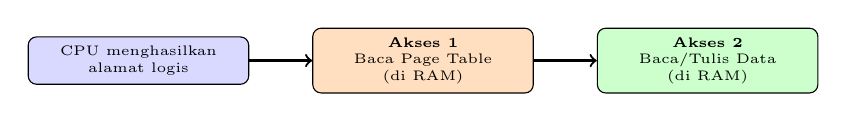
\begin{tikzpicture}[
            node distance=0.6cm,
            box/.style={draw, rounded corners=3pt, minimum width=2.8cm, minimum height=0.55cm, font=\tiny, align=center},
            arr/.style={->, thick}
        ]
            \node[box, fill=blue!15] (cpu)    {CPU menghasilkan\\alamat logis};
            \node[box, fill=orange!25, right=0.8cm of cpu] (pt) {\textbf{Akses 1}\\Baca Page Table\\(di RAM)};
            \node[box, fill=green!20, right=0.8cm of pt]  (data) {\textbf{Akses 2}\\Baca/Tulis Data\\(di RAM)};

            \draw[arr] (cpu) -- (pt);
            \draw[arr] (pt) -- (data);
        \end{tikzpicture}
    \end{block}

    \vspace{0.3cm}
    \begin{columns}[T]
        \column{0.48\textwidth}
        \textbf{Konsekuensinya:}
        \begin{itemize}
            \item Setiap instruksi yang mengakses memori $\rightarrow$ \tem{2 kali} baca RAM.
            \item Waktu akses efektif berlipat ganda.
            \item Semakin besar program, semakin besar page table-nya.
        \end{itemize}

        \column{0.48\textwidth}
        \begin{alertblock}{Ilustrasi}
            Jika akses RAM normal = \textbf{100 ns},\\
            maka dengan page table:\\
            $100 + 100 = $ \tem{200 ns} per akses logis.\\
            \vspace{0.1cm}
            Program lambat 2$\times$ hanya untuk translasi!
        \end{alertblock}
    \end{columns}
\end{frame}

\begin{frame}
    \frametitle{Visualisasi Overhead: Tanpa vs Dengan Optimasi}
    \framesubtitle{Perbandingan waktu akses memori}
    \small

    \begin{columns}[T]
        \column{0.48\textwidth}
        \textbf{Tanpa Optimasi (Page Table Biasa)}
        \vspace{0.2cm}

        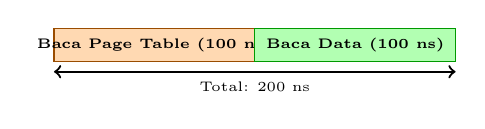
\begin{tikzpicture}[scale=0.85]
            \draw[fill=orange!30, draw=orange!60!black] (0,0) rectangle (3.0, 0.5) node[midway, font=\tiny\bfseries] {Baca Page Table (100 ns)};
            \draw[fill=green!30, draw=green!60!black]  (3.0,0) rectangle (6.0, 0.5) node[midway, font=\tiny\bfseries] {Baca Data (100 ns)};
            \draw[<->, thick] (0,-0.15) -- (6.0,-0.15) node[midway, below, font=\tiny] {Total: 200 ns};
        \end{tikzpicture}

        \vspace{0.5cm}
        \textbf{Dengan TLB (Hit)}
        \vspace{0.2cm}

        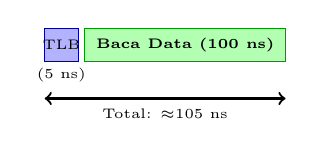
\begin{tikzpicture}[scale=0.85]
            \draw[fill=blue!30, draw=blue!60!black]   (0,0) rectangle (0.5, 0.5) node[midway, font=\tiny\bfseries] {};
            \node[font=\tiny] at (0.25, 0.25) {TLB};
            \node[font=\tiny] at (0.25, -0.2) {(5 ns)};
            \draw[fill=green!30, draw=green!60!black] (0.6,0) rectangle (3.6, 0.5) node[midway, font=\tiny\bfseries] {Baca Data (100 ns)};
            \draw[<->, thick] (0,-0.55) -- (3.6,-0.55) node[midway, below, font=\tiny] {Total: $\approx$105 ns};
        \end{tikzpicture}

        \column{0.48\textwidth}
        \begin{exampleblock}{Kenapa Jauh Lebih Cepat?}
            \begin{itemize}
                \item \textbf{TLB} adalah cache kecil dan \tem{sangat cepat} (chip CPU).
                \item Menyimpan entri page table yang baru-baru ini dipakai.
                \item Jika ditemukan di TLB (\textit{TLB hit}) $\rightarrow$ tidak perlu baca RAM untuk translasi.
                \item Program nyata: hit rate TLB bisa mencapai \tem{95--99\%}.
            \end{itemize}
        \end{exampleblock}
    \end{columns}
\end{frame}

\begin{frame}
    \frametitle{Solusi 1: TLB — Translation Lookaside Buffer}
    \framesubtitle{Cache untuk page table}
    \footnotesize

    \begin{block}{Definisi}
        TLB adalah \tem{cache asosiasif berkecepatan tinggi} yang menyimpan pasangan
        $\langle$\textit{page number}, \textit{frame number}$\rangle$ yang baru-baru ini digunakan.
    \end{block}

    \vspace{0.15cm}
    \begin{columns}[T]
        \column{0.48\textwidth}
        \textbf{TLB Hit} (\checkmark cepat)
        \begin{itemize}
            \item Page number ditemukan di TLB.
            \item Frame number langsung didapat.
            \item \tem{Tidak perlu} akses page table di RAM.
            \item Waktu: akses TLB + akses data.
        \end{itemize}

        \column{0.48\textwidth}
        \textbf{TLB Miss} ($\times$ lebih lambat)
        \begin{itemize}
            \item Page number \tem{tidak} ada di TLB.
            \item Harus baca page table di RAM.
            \item Entri baru dimuat ke TLB untuk akses berikutnya.
            \item Waktu: akses TLB + akses page table + akses data.
        \end{itemize}
    \end{columns}
\end{frame}

\begin{frame}
    \frametitle{Solusi 2: Demand Paging}
    \framesubtitle{Hanya muat page saat dibutuhkan}
    \footnotesize

    \begin{block}{Definisi}
        Demand paging adalah strategi di mana page \tem{tidak langsung dimuat ke RAM} saat proses
        dimulai, melainkan hanya dimuat \tem{saat pertama kali diakses}.
    \end{block}

    \vspace{0.15cm}
    \begin{columns}[T]
        \column{0.48\textwidth}
        \textbf{Page Hit} (\checkmark normal)
        \begin{itemize}
            \item Page yang diakses \tem{sudah ada} di RAM.
            \item Valid bit = 1 $\rightarrow$ translasi berjalan normal.
        \end{itemize}

        \vspace{0.2cm}
        \textbf{Page Fault} ($\times$ perlu penanganan)
        \begin{itemize}
            \item Page yang diakses \tem{belum ada} di RAM.
            \item Valid bit = 0 $\rightarrow$ OS harus muat dari disk.
            \item Jauh lebih lambat (ms vs ns).
        \end{itemize}

        \column{0.48\textwidth}
        \begin{exampleblock}{Keuntungan}
            \begin{itemize}
                \item RAM tidak terbuang untuk page yang tidak pernah dipakai.
                \item Proses bisa berjalan meski ukurannya lebih besar dari RAM fisik.
                \item Dasar dari \textit{virtual memory} modern.
            \end{itemize}
        \end{exampleblock}
    \end{columns}
\end{frame}

%================================================
% BAGIAN 2: TLB
%================================================
\section{TLB: Translation Lookaside Buffer}

\begin{frame}
    \frametitle{Apa Itu TLB?}
    \framesubtitle{Cache asosiasif untuk mempercepat translasi alamat}
    \small

    \begin{block}{Definisi}
        TLB (\textit{Translation Lookaside Buffer}) adalah \tem{cache berkecepatan tinggi} yang berada
        di dalam chip CPU, menyimpan pasangan $\langle$\textit{page number}, \textit{frame number}$\rangle$
        yang baru-baru ini digunakan.
    \end{block}

    \vspace{0.25cm}
    \begin{columns}[T]
        \column{0.48\textwidth}
        \textbf{Karakteristik TLB:}
        \begin{itemize}
            \item Berada di dalam atau dekat chip CPU.
            \item Kapasitas \tem{sangat kecil}: 16 -- 1024 entri.
            \item Kecepatan \tem{sangat tinggi}: 0.5 -- 5 ns.
            \item Pencarian dilakukan \tem{secara paralel} (asosiatif), bukan sekuensial seperti array.
        \end{itemize}

        \column{0.48\textwidth}
        \textbf{Isi setiap entri TLB:}

        \vspace{0.15cm}
        \begin{tabular}{|c|c|}
            \hline
            \textbf{Page \#} & \textbf{Frame \#} \\
            \hline
            3  & 7  \\
            \hline
            7  & 2  \\
            \hline
            12 & 0  \\
            \hline
            \ldots & \ldots \\
            \hline
        \end{tabular}

        \vspace{0.15cm}
        \footnotesize Entri lama diganti saat TLB penuh (\textit{replacement policy}).
    \end{columns}
\end{frame}

\begin{frame}
    \frametitle{Mekanisme: TLB Hit}
    \framesubtitle{Skenario terbaik — translasi tanpa akses RAM tambahan}
    \small

    \begin{block}{Kondisi: Page number ditemukan di TLB}
    \centering
    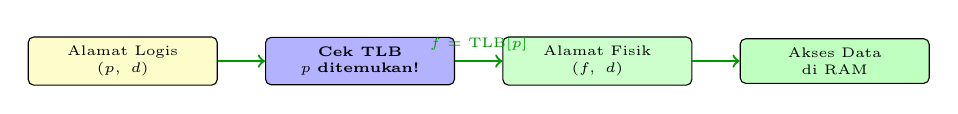
\begin{tikzpicture}[
        font=\tiny, node distance=0.5cm,
        box/.style={draw, rounded corners=2pt, minimum width=2.4cm, minimum height=0.55cm, align=center},
        arr/.style={->, thick, green!60!black}
    ]
        \node[box, fill=yellow!20] (la)   {Alamat Logis\\$(p,\ d)$};
        \node[box, fill=blue!30, right=0.6cm of la]   (tlb)  {\textbf{Cek TLB}\\$p$ \textbf{ditemukan!}};
        \node[box, fill=green!20, right=0.6cm of tlb] (fa)   {Alamat Fisik\\$(f,\ d)$};
        \node[box, fill=green!25, right=0.6cm of fa]  (data) {Akses Data\\di RAM};

        \draw[arr] (la)  -- (tlb);
        \draw[arr] (tlb) -- node[above, font=\tiny]{$f$ = TLB[$p$]} (fa);
        \draw[arr] (fa)  -- (data);
    \end{tikzpicture}
    \end{block}

    \vspace{0.2cm}
    \begin{columns}[T]
        \column{0.48\textwidth}
        \textbf{Langkah-langkah:}
        \begin{enumerate}
            \item CPU menghasilkan alamat logis $(p, d)$.
            \item TLB dicek: page $p$ \tem{ditemukan}.
            \item Frame number $f$ langsung diambil dari TLB.
            \item Alamat fisik $(f, d)$ digunakan untuk akses data.
        \end{enumerate}

        \column{0.48\textwidth}
        \begin{exampleblock}{Waktu Akses (TLB Hit)}
            \centering
            $T_{\text{hit}} = t_{\text{TLB}} + t_{\text{mem}}$

            \vspace{0.2cm}
            Contoh: $5 + 100 = \mathbf{105}$ \textbf{ns}

            \vspace{0.1cm}
            \footnotesize Jauh lebih cepat dari 200 ns\\tanpa TLB!
        \end{exampleblock}
    \end{columns}
\end{frame}

\begin{frame}
    \frametitle{Mekanisme: TLB Miss}
    \framesubtitle{Skenario penalti — harus akses page table di RAM}
    \small

    \begin{block}{Kondisi: Page number \textit{tidak} ditemukan di TLB}
    \centering
    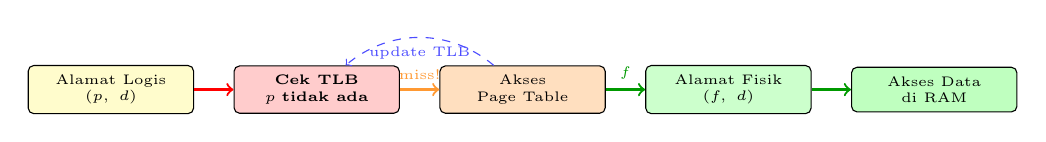
\begin{tikzpicture}[
        font=\tiny, node distance=0.45cm,
        box/.style={draw, rounded corners=2pt, minimum width=2.1cm, minimum height=0.55cm, align=center},
        arr/.style={->, thick}
    ]
        \node[box, fill=yellow!20] (la)   {Alamat Logis\\$(p,\ d)$};
        \node[box, fill=red!20, right=0.5cm of la]    (tlb)  {\textbf{Cek TLB}\\$p$ \textbf{tidak ada}};
        \node[box, fill=orange!25, right=0.5cm of tlb](pt)   {Akses\\Page Table};
        \node[box, fill=green!20, right=0.5cm of pt]  (fa)   {Alamat Fisik\\$(f,\ d)$};
        \node[box, fill=green!25, right=0.5cm of fa]  (data) {Akses Data\\di RAM};

        \draw[->, thick, red]           (la)  -- (tlb);
        \draw[->, thick, orange!80]     (tlb) -- node[above, font=\tiny]{miss!} (pt);
        \draw[->, thick, green!60!black](pt)  -- node[above, font=\tiny]{$f$} (fa);
        \draw[->, thick, green!60!black](fa)  -- (data);

        % Update TLB
        \draw[->, dashed, blue!70] (pt) to[bend right=40] node[below, font=\tiny]{update TLB} (tlb);
    \end{tikzpicture}
    \end{block}

    \vspace{0.15cm}
    \begin{columns}[T]
        \column{0.48\textwidth}
        \footnotesize\textbf{Langkah-langkah:}
        \begin{enumerate}
            \item CPU hasilkan alamat logis $(p, d)$.
            \item TLB dicek: $p$ \tem{tidak ditemukan} (miss).
            \item Akses page table di RAM $\rightarrow$ dapat $f$.
            \item Muat entri $(p, f)$ ke TLB.
            \item Akses data di RAM via $(f, d)$.
        \end{enumerate}

        \column{0.48\textwidth}
        \begin{alertblock}{Waktu Akses (TLB Miss)}
            \centering
            $T_{\text{miss}} = t_{\text{TLB}} + 2 \cdot t_{\text{mem}}$

            \vspace{0.15cm}
            Contoh: $5 + 200 = \mathbf{205}$ \textbf{ns}

            \vspace{0.1cm}
            \footnotesize Lebih lambat 2$\times$ dibanding TLB hit!
        \end{alertblock}
    \end{columns}
\end{frame}

\begin{frame}
    \frametitle{Diagram Alur: TLB Hit vs Miss}
    \framesubtitle{Perbandingan jalur eksekusi}
    \small

    \centering
    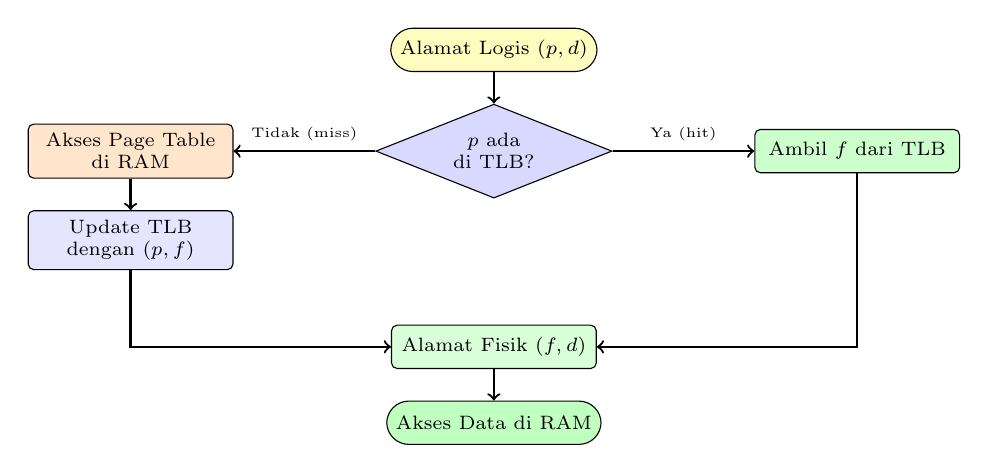
\begin{tikzpicture}[
        font=\scriptsize,
        decision/.style={draw, diamond, aspect=2.5, minimum width=3cm, minimum height=0.7cm, fill=blue!15, align=center},
        process/.style={draw, rounded corners=2pt, minimum width=2.6cm, minimum height=0.55cm, fill=gray!10, align=center},
        terminal/.style={draw, rounded corners=8pt, minimum width=2.6cm, minimum height=0.55cm, align=center},
        arr/.style={->, thick}
    ]
        \node[terminal, fill=yellow!25] (start) {Alamat Logis $(p, d)$};
        \node[decision, below=0.4cm of start] (check) {$p$ ada\\di TLB?};
        \node[process, fill=green!20, right=1.8cm of check] (hit) {Ambil $f$ dari TLB};
        \node[process, fill=orange!20, left=1.8cm of check] (miss) {Akses Page Table\\di RAM};
        \node[process, fill=blue!10, below=0.4cm of miss] (update) {Update TLB\\dengan $(p, f)$};
        \node[process, fill=green!15, below=1.6cm of check] (phys) {Alamat Fisik $(f, d)$};
        \node[terminal, fill=green!25, below=0.4cm of phys] (end) {Akses Data di RAM};

        \draw[arr] (start) -- (check);
        \draw[arr] (check) -- node[above, font=\tiny]{Ya (hit)} (hit);
        \draw[arr] (check) -- node[above, font=\tiny]{Tidak (miss)} (miss);
        \draw[arr] (miss)  -- (update);
        \draw[arr] (update) |- (phys);
        \draw[arr] (hit)    |- (phys);
        \draw[arr] (phys)  -- (end);
    \end{tikzpicture}
\end{frame}

\begin{frame}
    \frametitle{Effective Access Time (EAT)}
    \framesubtitle{Mengukur waktu rata-rata akses memori dengan TLB}
    \small

    \begin{block}{Rumus EAT}
        \centering
        \vspace{0.1cm}
        $\text{EAT} = \alpha \cdot (t_{\text{TLB}} + t_{\text{mem}}) + (1 - \alpha) \cdot (t_{\text{TLB}} + 2 \cdot t_{\text{mem}})$
        \vspace{0.1cm}
    \end{block}

    \vspace{0.2cm}
    \textbf{Keterangan variabel:}
    \begin{columns}[T]
        \column{0.48\textwidth}
        \begin{itemize}
            \item $\alpha$ = \textbf{TLB hit rate} (proporsi akses yang \textit{hit})
            \item $t_{\text{TLB}}$ = waktu akses TLB
            \item $t_{\text{mem}}$ = waktu akses RAM (1 kali)
        \end{itemize}

        \column{0.48\textwidth}
        \begin{itemize}
            \item Suku pertama: kontribusi \tem{TLB hit}
            \item Suku kedua: kontribusi \tem{TLB miss}\\(butuh 2 kali akses RAM)
        \end{itemize}
    \end{columns}

    \vspace{0.25cm}
    \begin{exampleblock}{Sederhanakan}
        \centering
        $\text{EAT} = t_{\text{TLB}} + t_{\text{mem}} + (1-\alpha) \cdot t_{\text{mem}}$

        \vspace{0.1cm}
        \footnotesize Semakin tinggi $\alpha$ (hit rate), semakin kecil EAT dan semakin cepat sistem!
    \end{exampleblock}
\end{frame}

\begin{frame}
    \frametitle{Contoh Perhitungan EAT}
    \framesubtitle{Sistem dengan hit rate 90\% dan 99\%}
    \small

    \textbf{Diketahui:} $t_{\text{TLB}} = 5$ ns, $t_{\text{mem}} = 100$ ns

    \vspace{0.3cm}
    \begin{columns}[T]
        \column{0.48\textwidth}
        \textbf{Kasus A: $\alpha = 0.90$ (90\%)}

        \vspace{0.1cm}
        \begin{align*}
            \text{EAT} &= 0.90 \times (5 + 100) \\
                       &\quad + 0.10 \times (5 + 200) \\
                       &= 0.90 \times 105 + 0.10 \times 205 \\
                       &= 94.5 + 20.5 \\
                       &= \mathbf{115\ ns}
        \end{align*}

        \column{0.48\textwidth}
        \textbf{Kasus B: $\alpha = 0.99$ (99\%)}

        \vspace{0.1cm}
        \begin{align*}
            \text{EAT} &= 0.99 \times (5 + 100) \\
                       &\quad + 0.01 \times (5 + 200) \\
                       &= 0.99 \times 105 + 0.01 \times 205 \\
                       &= 103.95 + 2.05 \\
                       &= \mathbf{106\ ns}
        \end{align*}
    \end{columns}

    \vspace{0.2cm}
    \begin{exampleblock}{Kesimpulan}
        Hit rate naik dari 90\% ke 99\% $\rightarrow$ EAT turun dari 115 ns ke 106 ns.\\
        Tanpa TLB sama sekali: $200$ ns. TLB \tem{sangat signifikan} pengaruhnya!
    \end{exampleblock}
\end{frame}

\begin{frame}
    \frametitle{Latihan: Hitung EAT}
    \framesubtitle{Kerjakan sebelum melihat solusi!}
    \small

    \begin{block}{Soal}
        Sebuah sistem memiliki spesifikasi berikut:
        \begin{itemize}
            \item Waktu akses TLB: $t_{\text{TLB}} = 10$ ns
            \item Waktu akses RAM: $t_{\text{mem}} = 150$ ns
            \item TLB hit rate: $\alpha = 0.95$
        \end{itemize}
        Hitunglah \textbf{Effective Access Time (EAT)} sistem tersebut!
    \end{block}

    \vspace{0.2cm}
    \begin{alertblock}{Rumus yang Digunakan}
        \centering
        $\text{EAT} = \alpha \cdot (t_{\text{TLB}} + t_{\text{mem}}) + (1-\alpha) \cdot (t_{\text{TLB}} + 2 \cdot t_{\text{mem}})$
    \end{alertblock}
\end{frame}

\begin{frame}
    \frametitle{Solusi Latihan EAT}
    \framesubtitle{Pembahasan langkah demi langkah}
    \small

    \textbf{Diketahui:} $t_{\text{TLB}} = 10$ ns, $t_{\text{mem}} = 150$ ns, $\alpha = 0.95$

    \vspace{0.2cm}
    \begin{columns}[T]
        \column{0.52\textwidth}
        \textbf{Langkah 1 — Hitung $T_{\text{hit}}$:}
        \[ T_{\text{hit}} = t_{\text{TLB}} + t_{\text{mem}} = 10 + 150 = 160 \text{ ns} \]

        \textbf{Langkah 2 — Hitung $T_{\text{miss}}$:}
        \[ T_{\text{miss}} = t_{\text{TLB}} + 2 \cdot t_{\text{mem}} = 10 + 300 = 310 \text{ ns} \]

        \textbf{Langkah 3 — Hitung EAT:}
        \begin{align*}
            \text{EAT} &= 0.95 \times 160 + 0.05 \times 310 \\
                       &= 152 + 15.5 \\
                       &= \mathbf{167.5 \text{ ns}}
        \end{align*}

        \column{0.44\textwidth}
        \begin{exampleblock}{Perbandingan}
            \begin{tabular}{lc}
                \hline
                \textbf{Kondisi} & \textbf{Waktu} \\
                \hline
                Tanpa TLB & 300 ns \\
                EAT ($\alpha=0.95$) & 167.5 ns \\
                TLB hit penuh & 160 ns \\
                \hline
            \end{tabular}

            \vspace{0.2cm}
            \footnotesize TLB menghemat \tem{$\approx$44\%} waktu akses dibanding tanpa TLB!
        \end{exampleblock}
    \end{columns}
\end{frame}

\begin{frame}
    \frametitle{TLB dan Context Switch}
    \framesubtitle{Apa yang terjadi saat proses berganti?}
    \small

    \begin{alertblock}{Masalah}
        TLB menyimpan entri milik proses yang sedang berjalan. Saat \tem{context switch} terjadi,
        entri TLB dari proses lama \tem{tidak berlaku} untuk proses baru!
    \end{alertblock}

    \vspace{0.2cm}
    \begin{columns}[T]
        \column{0.48\textwidth}
        \textbf{Solusi 1: TLB Flush}
        \begin{itemize}
            \item Seluruh isi TLB dikosongkan saat context switch.
            \item Sederhana, tapi proses baru mulai dari \tem{miss semua}.
            \item Perlu waktu untuk mengisi ulang TLB.
        \end{itemize}

        \column{0.48\textwidth}
        \textbf{Solusi 2: ASID (Address Space ID)}
        \begin{itemize}
            \item Setiap entri TLB diberi tag \tem{ID proses (ASID)}.
            \item TLB bisa menyimpan entri dari \tem{banyak proses} sekaligus.
            \item Hanya entri dengan ASID yang cocok yang dianggap valid.
            \item Lebih efisien, tidak perlu flush penuh.
        \end{itemize}
    \end{columns}
\end{frame}

\begin{frame}
    \frametitle{Checkpoint Pemahaman: TLB}
    \framesubtitle{Cek sebelum lanjut}
    \small

    \begin{enumerate}
        \item Apa perbedaan antara TLB hit dan TLB miss? Mana yang lebih cepat dan kenapa?
        \vspace{0.1cm}
        \item Jika hit rate TLB = 80\%, $t_{\text{TLB}}$ = 2 ns, $t_{\text{mem}}$ = 100 ns, berapa EAT-nya?
        \vspace{0.1cm}
        \item Mengapa TLB perlu di-\textit{flush} saat context switch terjadi?
        \vspace{0.1cm}
        \item Apa keuntungan menggunakan ASID dibandingkan TLB flush biasa?
        \vspace{0.1cm}
        \item Jika TLB penuh dan ada entri baru yang harus dimasukkan, apa yang terjadi?
    \end{enumerate}

    \vspace{0.2cm}
    \begin{block}{Jawaban Singkat}
        Jika Anda bisa menjawab semua dengan percaya diri, Anda siap untuk Bagian 3: Demand Paging!
    \end{block}
\end{frame}

%================================================
% BAGIAN 3: DEMAND PAGING
%================================================
\section{Demand Paging}

\begin{frame}
    \frametitle{Apa Itu Demand Paging?}
    \framesubtitle{Muat page hanya saat benar-benar dibutuhkan}
    \small

    \begin{block}{Definisi}
        Demand paging adalah strategi di mana page \tem{tidak dimuat ke RAM saat proses dimulai},
        melainkan hanya dimuat \tem{saat pertama kali diakses} oleh proses.
    \end{block}

    \vspace{0.2cm}
    \begin{columns}[T]
        \column{0.48\textwidth}
        \textbf{Tanpa Demand Paging:}
        \begin{itemize}
            \item Semua page proses dimuat ke RAM saat start.
            \item Boros memori — banyak page yang tidak pernah diakses.
            \item Proses besar tidak bisa berjalan jika RAM tidak cukup.
        \end{itemize}

        \column{0.48\textwidth}
        \textbf{Dengan Demand Paging:}
        \begin{itemize}
            \item Hanya page yang \tem{dibutuhkan} yang ada di RAM.
            \item RAM lebih efisien digunakan.
            \item Proses bisa berjalan meski ukurannya \tem{melebihi RAM fisik}.
            \item Dasar dari \textit{virtual memory} modern.
        \end{itemize}
    \end{columns}
\end{frame}

\begin{frame}
    \frametitle{Valid/Invalid Bit}
    \framesubtitle{Penanda apakah page sedang ada di RAM atau tidak}
    \small

    \begin{columns}[T]
        \column{0.52\textwidth}
        \begin{block}{Format Page Table dengan Valid Bit}
            \begin{tabular}{|c|c|c|l|}
                \hline
                \textbf{Page \#} & \textbf{Frame \#} & \textbf{V/I} & \textbf{Status} \\
                \hline
                0 & 4  & V & Ada di RAM \\
                \hline
                1 & -- & I & Tidak di RAM \\
                \hline
                2 & 7  & V & Ada di RAM \\
                \hline
                3 & -- & I & Tidak di RAM \\
                \hline
                4 & 1  & V & Ada di RAM \\
                \hline
            \end{tabular}
        \end{block}

        \column{0.44\textwidth}
        \textbf{Arti bit:}
        \begin{itemize}
            \item \textbf{V (Valid = 1):} Page ada di RAM, translasi bisa dilanjutkan.
            \item \textbf{I (Invalid = 0):} Page \tem{tidak ada di RAM} — terjadi \textit{page fault}, OS harus turun tangan.
        \end{itemize}

        \vspace{0.2cm}
        \begin{alertblock}{Perhatian}
            Invalid bukan berarti alamat salah! Bisa jadi page-nya memang valid tapi belum dimuat ke RAM.
        \end{alertblock}
    \end{columns}
\end{frame}

\begin{frame}
    \frametitle{Page Hit — Alur Akses Normal}
    \framesubtitle{Ketika page yang diakses sudah ada di RAM}
    \small

    \begin{block}{Kondisi: Valid bit = 1}
    \centering
    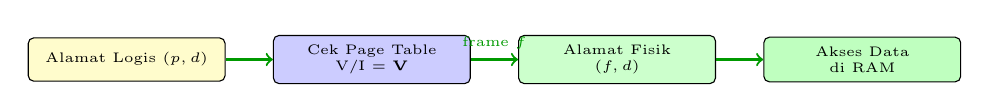
\begin{tikzpicture}[
        font=\tiny, node distance=0.5cm,
        box/.style={draw, rounded corners=2pt, minimum width=2.5cm, minimum height=0.55cm, align=center},
        arr/.style={->, thick, green!60!black}
    ]
        \node[box, fill=yellow!20] (la)  {Alamat Logis $(p, d)$};
        \node[box, fill=blue!20,  right=0.6cm of la]  (pt)   {Cek Page Table\\V/I = \textbf{V}};
        \node[box, fill=green!20, right=0.6cm of pt]  (fa)   {Alamat Fisik\\$(f, d)$};
        \node[box, fill=green!25, right=0.6cm of fa]  (data) {Akses Data\\di RAM};

        \draw[arr] (la) -- (pt);
        \draw[arr] (pt) -- node[above, font=\tiny]{frame $f$} (fa);
        \draw[arr] (fa) -- (data);
    \end{tikzpicture}
    \end{block}

    \vspace{0.25cm}
    \begin{columns}[T]
        \column{0.48\textwidth}
        \textbf{Langkah-langkah:}
        \begin{enumerate}
            \item CPU hasilkan alamat logis $(p, d)$.
            \item Cek page table: valid bit = \textbf{V}.
            \item Frame number $f$ diperoleh.
            \item Akses data di RAM via $(f, d)$.
        \end{enumerate}

        \column{0.48\textwidth}
        \begin{exampleblock}{Catatan}
            Page hit adalah skenario \tem{normal dan cepat}. Tidak ada intervensi OS — semua ditangani oleh hardware (MMU).
        \end{exampleblock}
    \end{columns}
\end{frame}

\begin{frame}
    \frametitle{Page Fault — Alur Penanganan}
    \framesubtitle{Ketika page yang diakses belum ada di RAM}
    \small

    \begin{block}{Kondisi: Valid bit = 0 $\rightarrow$ OS mengambil alih}
    \centering
    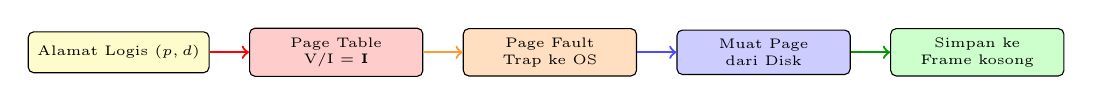
\begin{tikzpicture}[
        font=\tiny, node distance=0.45cm,
        box/.style={draw, rounded corners=2pt, minimum width=2.2cm, minimum height=0.52cm, align=center},
        arr/.style={->, thick}
    ]
        \node[box, fill=yellow!20] (la)   {Alamat Logis $(p,d)$};
        \node[box, fill=red!20,   right=0.5cm of la]  (pt)   {Page Table\\V/I = \textbf{I}};
        \node[box, fill=orange!25,right=0.5cm of pt]  (trap) {Page Fault\\Trap ke OS};
        \node[box, fill=blue!20,  right=0.5cm of trap](disk) {Muat Page\\dari Disk};
        \node[box, fill=green!20, right=0.5cm of disk](ram)  {Simpan ke\\Frame kosong};

        \draw[->, thick, red]         (la)   -- (pt);
        \draw[->, thick, orange!80]   (pt)   -- (trap);
        \draw[->, thick, blue!70]     (trap) -- (disk);
        \draw[->, thick, green!60!black](disk) -- (ram);
    \end{tikzpicture}
    \end{block}

    \vspace{0.15cm}
    \begin{columns}[T]
        \column{0.52\textwidth}
        \footnotesize\textbf{Langkah-langkah:}
        \begin{enumerate}
            \item MMU deteksi valid bit = I $\rightarrow$ \textit{page fault trap}.
            \item OS simpan state proses yang sedang berjalan.
            \item OS cari frame kosong di RAM.
            \item OS muat page dari disk ke frame tersebut.
            \item Update page table: set valid bit = V, isi frame \#.
            \item Restart instruksi yang tadi gagal.
        \end{enumerate}

        \column{0.44\textwidth}
        \begin{alertblock}{Mengapa Lambat?}
            Akses disk jauh lebih lambat dari RAM:
            \begin{itemize}
                \item RAM: $\sim$100 ns
                \item SSD: $\sim$100.000 ns
                \item HDD: $\sim$10.000.000 ns
            \end{itemize}
            Page fault $\rightarrow$ penalti \tem{besar}!
        \end{alertblock}
    \end{columns}
\end{frame}

\begin{frame}
    \frametitle{Diagram Alur: Page Fault Handler}
    \framesubtitle{Langkah OS dari deteksi hingga resume proses}
    \small

    \centering
    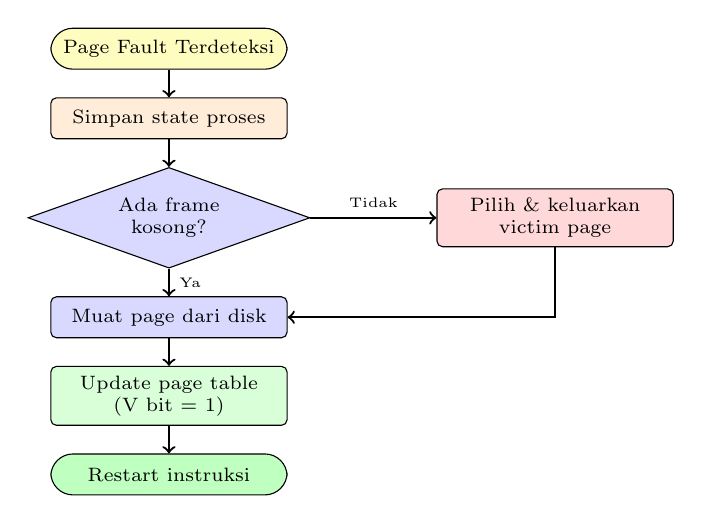
\begin{tikzpicture}[
        font=\scriptsize,
        decision/.style={draw, diamond, aspect=2.8, minimum width=3.2cm, minimum height=0.7cm, fill=blue!15, align=center},
        process/.style={draw, rounded corners=2pt, minimum width=3.0cm, minimum height=0.52cm, fill=gray!10, align=center},
        terminal/.style={draw, rounded corners=8pt, minimum width=3.0cm, minimum height=0.52cm, align=center},
        arr/.style={->, thick}
    ]
        \node[terminal, fill=yellow!25] (fault) {Page Fault Terdeteksi};
        \node[process,  fill=orange!15, below=0.35cm of fault]  (save)  {Simpan state proses};
        \node[decision, below=0.35cm of save]   (free)  {Ada frame\\kosong?};
        \node[process,  fill=red!15, right=1.6cm of free]  (evict) {Pilih \& keluarkan\\victim page};
        \node[process,  fill=blue!15, below=0.35cm of free] (load)  {Muat page dari disk};
        \node[process,  fill=green!15, below=0.35cm of load] (update){Update page table\\(V bit = 1)};
        \node[terminal, fill=green!25, below=0.35cm of update] (resume){Restart instruksi};

        \draw[arr] (fault)  -- (save);
        \draw[arr] (save)   -- (free);
        \draw[arr] (free)   -- node[right, font=\tiny]{Ya} (load);
        \draw[arr] (free)   -- node[above, font=\tiny]{Tidak} (evict);
        \draw[arr] (evict)  |- (load);
        \draw[arr] (load)   -- (update);
        \draw[arr] (update) -- (resume);
    \end{tikzpicture}
\end{frame}

\begin{frame}
    \frametitle{Contoh: Trace Akses Memori}
    \framesubtitle{Simulasi urutan akses dengan page fault}
    \footnotesize

    \textbf{Kondisi awal:} 3 frame kosong. Urutan akses page: \tem{1, 2, 3, 1, 4, 1}

    \vspace{0.15cm}
    \begin{columns}[T]
        \column{0.58\textwidth}
        \begin{tabular}{|c|c|c|c|c|c|}
            \hline
            \textbf{Ke-} & \textbf{Page} & \textbf{F0} & \textbf{F1} & \textbf{F2} & \textbf{Fault?} \\
            \hline
            1 & 1 & \cellcolor{green!25}P.1 & --  & --  & \cellcolor{green!25}Ya \\
            \hline
            2 & 2 & P.1 & \cellcolor{green!25}P.2 & --  & \cellcolor{green!25}Ya \\
            \hline
            3 & 3 & P.1 & P.2 & \cellcolor{green!25}P.3 & \cellcolor{green!25}Ya \\
            \hline
            4 & 1 & P.1 & P.2 & P.3 & Tidak \\
            \hline
            5 & 4 & \cellcolor{red!20}P.4 & P.2 & P.3 & \cellcolor{red!20}Ya \\
            \hline
            6 & 1 & P.4 & P.2 & \cellcolor{orange!25}P.1 & \cellcolor{orange!25}Ya \\
            \hline
        \end{tabular}

        \column{0.38\textwidth}
        \textbf{Keterangan:}
        \begin{itemize}
            \item \colorbox{green!25}{Hijau}: fault, frame kosong
            \item \colorbox{red!20}{Merah}: fault, ganti page lama
            \item \colorbox{orange!25}{Oranye}: fault, dimuat ulang
            \item Tanpa warna: page hit
        \end{itemize}

        \vspace{0.15cm}
        \begin{alertblock}{Hasil}
            Total akses: 6 \\
            \tem{Page fault: 5} \\
            Page hit: 1 \\
            (akses ke-4, page 1)
        \end{alertblock}
    \end{columns}
\end{frame}

\begin{frame}
    \frametitle{Pure Demand Paging vs Pre-paging}
    \framesubtitle{Dua pendekatan dalam memuat page ke memori}
    \small

    \begin{columns}[T]
        \column{0.48\textwidth}
        \textbf{Pure Demand Paging}
        \begin{itemize}
            \item Page \tem{hanya dimuat} saat terjadi page fault.
            \item Tidak ada page di RAM saat proses dimulai.
            \item Hemat memori, tapi banyak page fault di awal (\textit{cold start}).
            \item Cocok untuk proses yang besar dengan pola akses tidak menentu.
        \end{itemize}

        \column{0.48\textwidth}
        \textbf{Pre-paging}
        \begin{itemize}
            \item Beberapa page dimuat \tem{sebelum dibutuhkan} (prediksi).
            \item Mengurangi page fault di awal.
            \item Bisa boros jika prediksi salah.
            \item Cocok jika pola akses dapat diprediksi (misal: sequential).
        \end{itemize}
    \end{columns}
\end{frame}

\begin{frame}
    \frametitle{Checkpoint Pemahaman: Demand Paging}
    \framesubtitle{Cek sebelum lanjut}
    \small

    \begin{enumerate}
        \item Apa perbedaan antara page hit dan page fault? Mana yang lebih cepat dan kenapa?
        \vspace{0.1cm}
        \item Apa fungsi valid/invalid bit dalam page table?
        \vspace{0.1cm}
        \item Sebutkan 6 langkah yang dilakukan OS saat menangani page fault!
        \vspace{0.1cm}
        \item Mengapa page fault sangat mahal (lambat) dibanding page hit?
        \vspace{0.1cm}
        \item Apa perbedaan antara pure demand paging dan pre-paging?
    \end{enumerate}

    \vspace{0.2cm}
    \begin{block}{Jawaban Singkat}
        Jika Anda bisa menjawab semua dengan percaya diri, Anda siap untuk Bagian 4: Page Replacement!
    \end{block}
\end{frame}

%================================================
% BAGIAN 4: PAGE REPLACEMENT
%================================================
\section{Page Replacement}

\begin{frame}
    \frametitle{Masalah: Frame Penuh}
    \framesubtitle{Harus ganti page mana saat semua frame terisi?}
    \footnotesize

    \begin{alertblock}{Situasi}
        Page fault terjadi, tapi \tem{tidak ada frame kosong}. OS harus memilih satu page
        yang ada di RAM untuk \textbf{dikeluarkan} (\textit{victim page}) agar framenya bisa dipakai.
    \end{alertblock}

    \vspace{0.15cm}
    \begin{columns}[T]
        \column{0.50\textwidth}
        \textbf{Alur lengkap dengan replacement:}
        \begin{enumerate}
            \item Page fault terdeteksi.
            \item Tidak ada frame kosong.
            \item OS pilih \textit{victim page} berdasarkan algoritma.
            \item Tulis victim ke disk jika \textit{dirty} (\textit{swap out}).
            \item Muat page baru dari disk (\textit{swap in}).
            \item Update page table, restart instruksi.
        \end{enumerate}

        \column{0.46\textwidth}
        \begin{block}{Tujuan Algoritma Replacement}
            Memilih victim page yang \tem{paling jarang dibutuhkan} di masa depan, sehingga page fault seminimal mungkin.
        \end{block}

        \vspace{0.1cm}
        \textbf{Tiga algoritma utama:}
        \begin{itemize}
            \item FIFO (\textit{First In, First Out})
            \item Optimal (OPT)
            \item LRU (\textit{Least Recently Used})
        \end{itemize}
    \end{columns}
\end{frame}

\begin{frame}
    \frametitle{Konsep: Victim Page \& Dirty Bit}
    \framesubtitle{Detail teknis saat mengganti page}
    \footnotesize

    \begin{columns}[T]
        \column{0.52\textwidth}
        \begin{block}{Victim Page}
            Page yang dipilih untuk \textbf{dikeluarkan} dari RAM. Dipilih oleh algoritma page replacement.
        \end{block}

        \vspace{0.1cm}
        \begin{block}{Dirty Bit (Modified Bit)}
            Bit yang menandakan apakah page \tem{telah dimodifikasi} sejak terakhir dimuat.
            \begin{itemize}
                \item \textbf{Dirty = 0:} Sama dengan salinan di disk $\rightarrow$ langsung buang.
                \item \textbf{Dirty = 1:} Sudah berubah $\rightarrow$ \tem{harus ditulis ke disk} dulu.
            \end{itemize}
        \end{block}

        \column{0.44\textwidth}
        \begin{exampleblock}{Mengapa Dirty Bit Penting?}
            Menulis ke disk sangat lambat. Dengan dirty bit, OS bisa \tem{skip penulisan yang tidak perlu} jika page tidak dimodifikasi.
        \end{exampleblock}

        \vspace{0.15cm}
        \begin{tabular}{|c|c|c|c|}
            \hline
            \textbf{Page} & \textbf{Frame} & \textbf{Valid} & \textbf{Dirty} \\
            \hline
            0 & 3 & V & 0 \\
            \hline
            1 & 7 & V & 1 \\
            \hline
            2 & -- & I & 0 \\
            \hline
        \end{tabular}
    \end{columns}
\end{frame}

\begin{frame}
    \frametitle{Algoritma FIFO}
    \framesubtitle{Ganti page yang paling lama berada di RAM}
    \footnotesize

    \begin{block}{Prinsip}
        Keluarkan page yang \tem{pertama kali masuk} ke RAM. Page yang paling lama di memori dijadikan victim.
    \end{block}

    \vspace{0.1cm}
    \textbf{Contoh:} 3 frame, urutan akses: \tem{7, 0, 1, 2, 0, 3, 0, 4, 2, 3}

    \vspace{0.1cm}
    \begin{tabular}{|c|c|c|c|c|c|c|c|c|c|c|}
        \hline
        \textbf{Akses} & 7 & 0 & 1 & 2 & 0 & 3 & 0 & 4 & 2 & 3 \\
        \hline
        \textbf{F0} & \cellcolor{green!20}7 & 7 & 7 & \cellcolor{red!20}2 & 2 & 2 & 2 & \cellcolor{red!20}4 & 4 & 4 \\
        \hline
        \textbf{F1} & -- & \cellcolor{green!20}0 & 0 & 0 & 0 & \cellcolor{red!20}3 & 3 & 3 & \cellcolor{red!20}2 & 2 \\
        \hline
        \textbf{F2} & -- & -- & \cellcolor{green!20}1 & 1 & 1 & 1 & 1 & 1 & 1 & \cellcolor{red!20}3 \\
        \hline
        \textbf{Fault?} & \cellcolor{green!20}Ya & \cellcolor{green!20}Ya & \cellcolor{green!20}Ya & \cellcolor{red!20}Ya & -- & \cellcolor{red!20}Ya & -- & \cellcolor{red!20}Ya & \cellcolor{red!20}Ya & \cellcolor{red!20}Ya \\
        \hline
    \end{tabular}

    \vspace{0.1cm}
    \begin{columns}[T]
        \column{0.48\textwidth}
        \begin{itemize}
            \item \colorbox{green!20}{Hijau}: fault, frame kosong.
            \item \colorbox{red!20}{Merah}: fault, ganti page lama.
            \item Tanpa warna: page hit.
        \end{itemize}

        \column{0.48\textwidth}
        \begin{alertblock}{Hasil FIFO}
            \textbf{Page fault: 9 dari 10.}\\
            Sederhana tapi sering tidak optimal.
        \end{alertblock}
    \end{columns}
\end{frame}

\begin{frame}
    \frametitle{Belady's Anomaly}
    \framesubtitle{Fenomena aneh pada algoritma FIFO}
    \footnotesize

    \begin{alertblock}{Anomali Belady}
        Pada algoritma FIFO, \tem{menambah jumlah frame} terkadang justru \tem{meningkatkan} jumlah page fault — berlawanan dengan intuisi!
    \end{alertblock}

    \vspace{0.15cm}
    \textbf{Contoh dengan urutan akses: 1, 2, 3, 4, 1, 2, 5, 1, 2, 3, 4, 5}

    \vspace{0.1cm}
    \begin{columns}[T]
        \column{0.48\textwidth}
        \begin{block}{3 Frame $\rightarrow$ \textbf{9 page fault}}
            Frame selalu penuh dan sering tergantikan karena ruang terbatas.
        \end{block}

        \column{0.48\textwidth}
        \begin{block}{4 Frame $\rightarrow$ \textbf{10 page fault}}
            Lebih banyak frame, tapi urutan penggantian FIFO menjadi kurang beruntung — lebih banyak fault!
        \end{block}
    \end{columns}

    \vspace{0.15cm}
    \begin{exampleblock}{Implikasi}
        Belady's anomaly hanya terjadi pada FIFO. Algoritma \tem{OPT dan LRU tidak mengalami anomali} ini karena termasuk algoritma \textit{stack-based}.
    \end{exampleblock}
\end{frame}

\begin{frame}
    \frametitle{Algoritma Optimal (OPT)}
    \framesubtitle{Ganti page yang paling lama tidak akan digunakan}
    \footnotesize

    \begin{block}{Prinsip}
        Keluarkan page yang \tem{paling jauh dibutuhkan di masa depan}. Menghasilkan page fault paling sedikit, tapi \tem{tidak bisa diimplementasikan} di sistem nyata (butuh pengetahuan masa depan). Digunakan sebagai acuan ideal.
    \end{block}

    \vspace{0.1cm}
    \textbf{Contoh:} 3 frame, urutan akses: \tem{7, 0, 1, 2, 0, 3, 0, 4, 2, 3}

    \vspace{0.1cm}
    \begin{tabular}{|c|c|c|c|c|c|c|c|c|c|c|}
        \hline
        \textbf{Akses} & 7 & 0 & 1 & 2 & 0 & 3 & 0 & 4 & 2 & 3 \\
        \hline
        \textbf{F0} & \cellcolor{green!20}7 & 7 & 7 & \cellcolor{red!20}2 & 2 & 2 & 2 & 2 & 2 & 2 \\
        \hline
        \textbf{F1} & -- & \cellcolor{green!20}0 & 0 & 0 & 0 & 0 & 0 & \cellcolor{red!20}4 & 4 & \cellcolor{red!20}3 \\
        \hline
        \textbf{F2} & -- & -- & \cellcolor{green!20}1 & 1 & 1 & \cellcolor{red!20}3 & 3 & 3 & 3 & 3 \\
        \hline
        \textbf{Fault?} & \cellcolor{green!20}Ya & \cellcolor{green!20}Ya & \cellcolor{green!20}Ya & \cellcolor{red!20}Ya & -- & \cellcolor{red!20}Ya & -- & \cellcolor{red!20}Ya & -- & -- \\
        \hline
    \end{tabular}

    \vspace{0.1cm}
    \begin{columns}[T]
        \column{0.58\textwidth}
        \textbf{Victim dipilih} dengan melihat ke depan: ganti page yang \textit{next use}-nya paling jauh.

        \column{0.38\textwidth}
        \begin{exampleblock}{Hasil OPT}
            \textbf{Page fault: 6 dari 10.}\\
            Lebih baik dari FIFO (9)!
        \end{exampleblock}
    \end{columns}
\end{frame}

\begin{frame}
    \frametitle{Algoritma LRU}
    \framesubtitle{Ganti page yang paling lama tidak digunakan}
    \footnotesize

    \begin{block}{Prinsip}
        Keluarkan page yang \tem{terakhir kali digunakan paling lama yang lalu}. LRU menggunakan history penggunaan sebagai aproksimasi masa depan dan \tem{bisa diimplementasikan} di sistem nyata.
    \end{block}

    \vspace{0.1cm}
    \textbf{Contoh:} 3 frame, urutan akses: \tem{7, 0, 1, 2, 0, 3, 0, 4, 2, 3}

    \vspace{0.1cm}
    \begin{tabular}{|c|c|c|c|c|c|c|c|c|c|c|}
        \hline
        \textbf{Akses} & 7 & 0 & 1 & 2 & 0 & 3 & 0 & 4 & 2 & 3 \\
        \hline
        \textbf{F0} & \cellcolor{green!20}7 & 7 & 7 & \cellcolor{red!20}2 & 2 & 2 & 2 & \cellcolor{red!20}4 & 4 & \cellcolor{red!20}3 \\
        \hline
        \textbf{F1} & -- & \cellcolor{green!20}0 & 0 & 0 & 0 & \cellcolor{red!20}3 & 3 & 3 & 3 & 3 \\
        \hline
        \textbf{F2} & -- & -- & \cellcolor{green!20}1 & 1 & 1 & 1 & 1 & 1 & \cellcolor{red!20}2 & 2 \\
        \hline
        \textbf{Fault?} & \cellcolor{green!20}Ya & \cellcolor{green!20}Ya & \cellcolor{green!20}Ya & \cellcolor{red!20}Ya & -- & \cellcolor{red!20}Ya & -- & \cellcolor{red!20}Ya & \cellcolor{red!20}Ya & \cellcolor{red!20}Ya \\
        \hline
    \end{tabular}

    \vspace{0.1cm}
    \begin{columns}[T]
        \column{0.58\textwidth}
        \textbf{Victim dipilih} berdasarkan timestamp: ganti page yang terakhir dipakai paling lama lalu.

        \column{0.38\textwidth}
        \begin{alertblock}{Hasil LRU}
            \textbf{Page fault: 8 dari 10.}\\
            Lebih baik dari FIFO, mendekati OPT.
        \end{alertblock}
    \end{columns}
\end{frame}

\begin{frame}
    \frametitle{Perbandingan: FIFO vs OPT vs LRU}
    \framesubtitle{Ringkasan tiga algoritma pada contoh yang sama}
    \small

    \textbf{Urutan akses:} \tem{7, 0, 1, 2, 0, 3, 0, 4, 2, 3} \quad|\quad \textbf{Frame:} 3

    \vspace{0.2cm}
    \begin{tabular}{|l|c|c|c|l|}
        \hline
        \textbf{Algoritma} & \textbf{Fault} & \textbf{Hit} & \textbf{Fault Rate} & \textbf{Catatan} \\
        \hline
        FIFO        & 9 & 1 & 90\% & Sederhana, rentan Belady's anomaly \\
        \hline
        Optimal (OPT) & 6 & 4 & 60\% & Terbaik, tidak realistis \\
        \hline
        LRU         & 8 & 2 & 80\% & Praktis, mendekati optimal \\
        \hline
    \end{tabular}

    \vspace{0.2cm}
    \begin{columns}[T]
        \column{0.48\textwidth}
        \begin{exampleblock}{Kesimpulan}
            \begin{itemize}
                \item \textbf{OPT} = batas bawah ideal (acuan).
                \item \textbf{LRU} = pilihan terbaik yang implementable.
                \item \textbf{FIFO} = paling mudah, tapi suboptimal.
            \end{itemize}
        \end{exampleblock}

        \column{0.48\textwidth}
        \begin{alertblock}{Di Sistem Nyata}
            LRU murni mahal (perlu timestamp tiap akses). OS modern menggunakan aproksimasi seperti \textbf{Clock Algorithm} atau \textbf{NFU}.
        \end{alertblock}
    \end{columns}
\end{frame}

\begin{frame}
    \frametitle{Latihan: Bandingkan Ketiga Algoritma}
    \framesubtitle{Hitung page fault untuk FIFO, OPT, dan LRU}
    \footnotesize

    \begin{block}{Soal}
        Diberikan \textbf{4 frame} (awalnya kosong) dan urutan akses page:

        \vspace{0.1cm}
        \centering\tem{1, 2, 3, 4, 1, 2, 5, 1, 2, 3, 4, 5}
    \end{block}

    \vspace{0.15cm}
    Untuk masing-masing algoritma (\textbf{FIFO}, \textbf{OPT}, \textbf{LRU}):
    \begin{enumerate}
        \item Trace isi frame setiap langkah.
        \item Tandai setiap page fault.
        \item Hitung total page fault.
    \end{enumerate}

    \vspace{0.1cm}
    \begin{alertblock}{Petunjuk}
        \begin{itemize}
            \item \textbf{FIFO:} Ganti page yang paling lama masuk (antrian).
            \item \textbf{OPT:} Ganti page yang berikutnya dipakai paling jauh ke depan.
            \item \textbf{LRU:} Ganti page yang terakhir dipakai paling lama ke belakang.
        \end{itemize}
    \end{alertblock}
\end{frame}

%================================================
% BAGIAN 5: LATIHAN TERPADU
%================================================
\section{Latihan Terpadu}

\begin{frame}
    \frametitle{Latihan 1: Hitung EAT}
    \framesubtitle{Kerjakan sebelum melihat solusi!}
    \footnotesize

    \begin{block}{Soal}
        Sebuah sistem memori memiliki spesifikasi berikut:
        \begin{itemize}
            \item Waktu akses TLB: $t_{\text{TLB}} = 20$ ns
            \item Waktu akses RAM: $t_{\text{mem}} = 200$ ns
            \item TLB hit rate: $\alpha = 0.80$
        \end{itemize}
        \textbf{(a)} Hitung EAT sistem tersebut.\\
        \textbf{(b)} Berapa EAT jika hit rate ditingkatkan menjadi 95\%?\\
        \textbf{(c)} Berapa EAT tanpa TLB sama sekali?
    \end{block}

    \vspace{0.15cm}
    \begin{alertblock}{Rumus}
        \centering
        $\text{EAT} = \alpha \cdot (t_{\text{TLB}} + t_{\text{mem}}) + (1-\alpha) \cdot (t_{\text{TLB}} + 2 \cdot t_{\text{mem}})$
    \end{alertblock}
\end{frame}

\begin{frame}
    \frametitle{Solusi Latihan 1}
    \framesubtitle{Pembahasan (a), (b), dan (c)}
    \footnotesize

    \textbf{Diketahui:} $t_{\text{TLB}} = 20$ ns, $t_{\text{mem}} = 200$ ns

    \vspace{0.1cm}
    \begin{columns}[T]
        \column{0.52\textwidth}
        \textbf{(a) $\alpha = 0.80$:}
        \begin{align*}
            T_{\text{hit}}  &= 20 + 200 = 220 \text{ ns}\\
            T_{\text{miss}} &= 20 + 400 = 420 \text{ ns}\\
            \text{EAT} &= 0.80 \times 220 + 0.20 \times 420\\
                       &= 176 + 84 = \mathbf{260 \text{ ns}}
        \end{align*}

        \textbf{(b) $\alpha = 0.95$:}
        \begin{align*}
            \text{EAT} &= 0.95 \times 220 + 0.05 \times 420\\
                       &= 209 + 21 = \mathbf{230 \text{ ns}}
        \end{align*}

        \textbf{(c) Tanpa TLB:}
        \[ \text{EAT} = 2 \times t_{\text{mem}} = \mathbf{400 \text{ ns}} \]

        \column{0.44\textwidth}
        \begin{exampleblock}{Perbandingan}
            \begin{tabular}{lc}
                \hline
                \textbf{Kondisi} & \textbf{EAT} \\
                \hline
                Tanpa TLB       & 400 ns \\
                TLB ($\alpha$=80\%) & 260 ns \\
                TLB ($\alpha$=95\%) & 230 ns \\
                TLB hit penuh   & 220 ns \\
                \hline
            \end{tabular}

            \vspace{0.15cm}
            TLB 80\% sudah hemat \tem{35\%} dibanding tanpa TLB. Naik ke 95\% hemat \tem{42.5\%}!
        \end{exampleblock}
    \end{columns}
\end{frame}

\begin{frame}
    \frametitle{Latihan 2: FIFO vs LRU}
    \framesubtitle{Trace page replacement dan bandingkan hasilnya}
    \footnotesize

    \begin{block}{Soal}
        Diberikan \textbf{3 frame} (awalnya kosong) dan urutan akses page:

        \vspace{0.1cm}
        \centering\tem{2, 3, 2, 1, 5, 2, 4, 5, 3, 2, 5, 2}
    \end{block}

    \vspace{0.15cm}
    \begin{columns}[T]
        \column{0.48\textwidth}
        Untuk algoritma \textbf{FIFO} dan \textbf{LRU}:
        \begin{enumerate}
            \item Trace isi frame setiap langkah.
            \item Tandai setiap page fault.
            \item Hitung total page fault masing-masing.
            \item Tentukan mana yang lebih efisien.
        \end{enumerate}

        \column{0.48\textwidth}
        \begin{alertblock}{Petunjuk}
            \begin{itemize}
                \item \textbf{FIFO:} Catat urutan masuknya page. Ganti yang paling pertama masuk.
                \item \textbf{LRU:} Catat kapan terakhir page diakses. Ganti yang paling lama tidak dipakai.
            \end{itemize}
        \end{alertblock}
    \end{columns}
\end{frame}

\begin{frame}
    \frametitle{Solusi Latihan 2: FIFO}
    \framesubtitle{Urutan akses: 2, 3, 2, 1, 5, 2, 4, 5, 3, 2, 5, 2}
    \footnotesize

    \begin{tabular}{|c|c|c|c|c|c|c|c|c|c|c|c|c|}
        \hline
        \textbf{Akses} & 2 & 3 & 2 & 1 & 5 & 2 & 4 & 5 & 3 & 2 & 5 & 2 \\
        \hline
        \textbf{F0} & \cellcolor{green!20}2 & 2 & 2 & 2 & \cellcolor{red!20}5 & 5 & 5 & 5 & \cellcolor{red!20}3 & 3 & 3 & 3 \\
        \hline
        \textbf{F1} & -- & \cellcolor{green!20}3 & 3 & 3 & 3 & 3 & \cellcolor{red!20}4 & 4 & 4 & \cellcolor{red!20}2 & 2 & 2 \\
        \hline
        \textbf{F2} & -- & -- & -- & \cellcolor{green!20}1 & 1 & 1 & 1 & 1 & 1 & 1 & \cellcolor{red!20}5 & 5 \\
        \hline
        \textbf{Fault?} & \cellcolor{green!20}Ya & \cellcolor{green!20}Ya & -- & \cellcolor{green!20}Ya & \cellcolor{red!20}Ya & -- & \cellcolor{red!20}Ya & -- & \cellcolor{red!20}Ya & \cellcolor{red!20}Ya & \cellcolor{red!20}Ya & -- \\
        \hline
    \end{tabular}

    \vspace{0.15cm}
    \begin{columns}[T]
        \column{0.48\textwidth}
        \begin{itemize}
            \item \colorbox{green!20}{Hijau}: fault, frame kosong.
            \item \colorbox{red!20}{Merah}: fault, ganti page lama.
            \item Tanpa warna: page hit.
        \end{itemize}

        \column{0.48\textwidth}
        \begin{alertblock}{Hasil FIFO}
            \textbf{Page fault: 9 dari 12 akses}\\
            Page hit: 3 (akses ke 3, 6, 12)
        \end{alertblock}
    \end{columns}
\end{frame}

\begin{frame}
    \frametitle{Solusi Latihan 2: LRU}
    \framesubtitle{Urutan akses: 2, 3, 2, 1, 5, 2, 4, 5, 3, 2, 5, 2}
    \footnotesize

    \begin{tabular}{|c|c|c|c|c|c|c|c|c|c|c|c|c|}
        \hline
        \textbf{Akses} & 2 & 3 & 2 & 1 & 5 & 2 & 4 & 5 & 3 & 2 & 5 & 2 \\
        \hline
        \textbf{F0} & \cellcolor{green!20}2 & 2 & 2 & 2 & 2 & 2 & \cellcolor{red!20}4 & 4 & \cellcolor{red!20}3 & \cellcolor{red!20}2 & 2 & 2 \\
        \hline
        \textbf{F1} & -- & \cellcolor{green!20}3 & 3 & 3 & \cellcolor{red!20}5 & 5 & 5 & 5 & 5 & 5 & 5 & 5 \\
        \hline
        \textbf{F2} & -- & -- & -- & \cellcolor{green!20}1 & 1 & 1 & 1 & 1 & 1 & 1 & \cellcolor{red!20}5 & 5 \\
        \hline
        \textbf{Fault?} & \cellcolor{green!20}Ya & \cellcolor{green!20}Ya & -- & \cellcolor{green!20}Ya & \cellcolor{red!20}Ya & -- & \cellcolor{red!20}Ya & -- & \cellcolor{red!20}Ya & \cellcolor{red!20}Ya & \cellcolor{red!20}Ya & -- \\
        \hline
    \end{tabular}

    \vspace{0.15cm}
    \begin{columns}[T]
        \column{0.48\textwidth}
        \begin{exampleblock}{Hasil LRU}
            \textbf{Page fault: 9 dari 12 akses}\\
            Page hit: 3 (akses ke 3, 6, 12)
        \end{exampleblock}

        \column{0.48\textwidth}
        \begin{block}{Kesimpulan}
            Pada kasus ini FIFO dan LRU menghasilkan jumlah page fault yang \tem{sama (9)}. Hasilnya bisa berbeda tergantung urutan akses dan jumlah frame.
        \end{block}
    \end{columns}
\end{frame}

%================================================
% BAGIAN 6: RINGKASAN & PENUTUP
%================================================
\section{Ringkasan}

\begin{frame}
    \frametitle{Ringkasan: Poin Kunci}
    \framesubtitle{Intisari materi pertemuan ini}
    \small

    \begin{columns}[T]
        \column{0.48\textwidth}
        \textbf{TLB \& EAT:}
        \begin{enumerate}
            \item Page table biasa butuh \tem{2 akses RAM} per translasi.
            \item TLB menyimpan entri terbaru secara \tem{asosiatif dan cepat}.
            \item \textbf{TLB hit} $\rightarrow$ $t_{\text{TLB}} + t_{\text{mem}}$.
            \item \textbf{TLB miss} $\rightarrow$ $t_{\text{TLB}} + 2t_{\text{mem}}$.
            \item $\text{EAT} = \alpha \cdot T_{\text{hit}} + (1-\alpha) \cdot T_{\text{miss}}$.
            \item Context switch $\rightarrow$ TLB flush atau ASID.
        \end{enumerate}

        \column{0.48\textwidth}
        \textbf{Demand Paging \& Page Replacement:}
        \begin{enumerate}
            \item Valid bit = 0 $\rightarrow$ \tem{page fault}, OS mengambil alih.
            \item Page fault mahal: harus akses disk (ms vs ns).
            \item Frame penuh $\rightarrow$ pilih \textit{victim} dengan algoritma.
            \item \textbf{FIFO}: sederhana, rentan Belady's anomaly.
            \item \textbf{OPT}: ideal tapi tidak bisa diimplementasikan.
            \item \textbf{LRU}: praktis dan mendekati optimal.
        \end{enumerate}
    \end{columns}
\end{frame}

\begin{frame}
    \frametitle{Checklist Keterampilan}
    \framesubtitle{Pastikan Anda dapat melakukan ini}
    \small

    \begin{columns}[T]
        \column{0.48\textwidth}
        \textbf{TLB \& EAT:}
        \begin{itemize}
            \item[$\square$] Menjelaskan perbedaan TLB hit dan TLB miss.
            \item[$\square$] Menghitung $T_{\text{hit}}$ dan $T_{\text{miss}}$ dari parameter yang diberikan.
            \item[$\square$] Menghitung EAT dari hit rate dan waktu akses.
            \item[$\square$] Menjelaskan peran ASID saat context switch.
        \end{itemize}

        \column{0.48\textwidth}
        \textbf{Demand Paging \& Page Replacement:}
        \begin{itemize}
            \item[$\square$] Membaca page table dan menentukan page hit/fault.
            \item[$\square$] Menjelaskan 6 langkah penanganan page fault oleh OS.
            \item[$\square$] Men-trace FIFO, OPT, dan LRU step-by-step.
            \item[$\square$] Membandingkan jumlah page fault ketiga algoritma.
        \end{itemize}
    \end{columns}
\end{frame}

\begin{frame}
    \frametitle{Terima Kasih}
    \begin{center}
        \Huge \textbf{Ada Pertanyaan?}

        \vspace{0.8cm}
        \normalsize
        Jika ada satu konsep yang belum jelas, jangan lanjut.\\
        Tanyakan sekarang atau diskusikan di forum kuliah.

        \vspace{0.8cm}
        \small
        \textit{``The art of doing mathematics consists in finding that special case\\
        which contains all the germs of generality.''} \\
        \vspace{0.1cm}
        --- David Hilbert
    \end{center}
\end{frame}

\end{document}
